\PassOptionsToPackage{subsection=false}{beamerouterthememiniframes}
\PassOptionsToPackage{dvipsnames,table}{xcolor}
\documentclass[fleqn]{beamer}
\usepackage{graphicx}
\usepackage{multirow}
\usepackage{multicol}
\usepackage{amsmath,amsfonts,amsthm,amsopn}
\usepackage{color, colortbl}
\usepackage{subfig}
\usepackage{wrapfig}
\usepackage{fancybox}
\usepackage{tikz}
\usepackage{fancyhdr}
\usepackage{setspace}
\usepackage{xcolor}
\usepackage{movie15}
\usepackage{pifont}
\usepackage{soul}
\usepackage{fancyvrb,newverbs}
\usepackage{epsfig}
\usepackage{epstopdf}
\fvset{fontsize=\footnotesize}
\RecustomVerbatimEnvironment{verbatim}{Verbatim}{}

%\usepackage{fancybox}

\usetheme{Szeged}
\usecolortheme{default}

%\definecolor{links}{HTML}{2A1B81}
%\definecolor{links}{blue!20}
\hypersetup{colorlinks,linkcolor=,urlcolor=blue!80}

\setbeamertemplate{blocks}[rounded]
\setbeamercolor{block title}{bg=blue!40,fg=black}
\setbeamercolor{block body}{bg=blue!10}


\newenvironment<>{clicker}[1]{%
  \begin{actionenv}#2%
      \def\insertblocktitle{#1}%
      \par%
      \mode<presentation>{%
        \setbeamercolor{block title}{fg=white,bg=magenta}
       \setbeamercolor{block body}{fg=black,bg=magenta!10}
       \setbeamercolor{itemize item}{fg=magenta}
       \setbeamertemplate{itemize item}[triangle]
       \setbeamercolor{enumerate item}{fg=magenta}
     }%
      \usebeamertemplate{block begin}}
    {\par\usebeamertemplate{block end}\end{actionenv}}

%\newcommand{\bmp}{\begin{minipage}}
%\newcommand{\emp}{\end{minipage}}
%\newcommand{\blankcolumn}{\bmp{.05\textwidth}\hspace{0.50in} \emp}

\defbeamertemplate*{footline}{infolines theme}
{
  \leavevmode%
  \hbox{%
  \begin{beamercolorbox}[wd=.333333\paperwidth,ht=2.25ex,dp=1ex,left]{author in head/foot}%
    \usebeamerfont{author in head/foot}~~\insertshortinstitute: \insertshorttitle
  \end{beamercolorbox}%
  \begin{beamercolorbox}[wd=.67\paperwidth,ht=2.25ex,dp=1ex,right]{date in head/foot}%
    \usebeamerfont{date in head/foot}%\insertshortdate{}\hspace*{2em}
    \insertframenumber{} / \inserttotalframenumber\hspace*{2ex}
  \end{beamercolorbox}
  }%
  \vskip0pt%
}

\newcommand{\cmark}{\ding{51}}%
\newcommand{\xmark}{\ding{55}}%
\newcommand{\grp}{\textcolor{magenta}{Group Exercise}}
\newcommand{\grpc}{\textcolor{magenta}{Group Exercise, continued}}
\newcommand{\bsans}[1]{\underline{\hspace{0.2in}\color{blue!80}{#1}\hspace{0.2in}}}

\definecolor{cverbbg}{gray}{0.93}
\newenvironment{cverbatim}
 {\SaveVerbatim{cverb}}
 {\endSaveVerbatim
  \flushleft\fboxrule=0pt\fboxsep=.5em
  \colorbox{cverbbg}{\BUseVerbatim{cverb}}%
  \endflushleft
}
\newenvironment{lcverbatim}
 {\SaveVerbatim{cverb}}
 {\endSaveVerbatim
  \flushleft\fboxrule=0pt\fboxsep=.5em
  \colorbox{cverbbg}{%
    \makebox[\dimexpr\linewidth-2\fboxsep][l]{\BUseVerbatim{cverb}}%
  }
  \endflushleft
}

\newcommand{\bmp}{\begin{minipage}}
\newcommand{\emp}{\end{minipage}}
\newcommand{\blankcolumn}{\bmp{.05\textwidth}\hspace{0.50in} \emp}

 \newenvironment{code}[1]%
  {\vspace{.1in}\footnotesize\Verbatim[frame=single,label=SAS Code,commandchars=\\\{\},xrightmargin=#1\textwidth,framesep=.2in,labelposition=all]}
  {\endVerbatim\normalsize}

 \newenvironment{Rcode}[1]%
  {\vspace{.1in}\footnotesize\Verbatim[frame=single,label=R Code,commandchars=\\\{\},xrightmargin=#1\textwidth,framesep=.2in,labelposition=all]}
  {\endVerbatim\normalsize}

   \newenvironment{RcodeScript}[1]%
  {\vspace{.1in}\scriptsize\Verbatim[frame=single,label=R Code,commandchars=\\\{\},xrightmargin=#1\textwidth,framesep=.2in,labelposition=all]}
  {\endVerbatim\normalsize}

 \newenvironment{RcodeTiny}[1]%
  {\vspace{.1in}\tiny\Verbatim[frame=single,label=R Code,commandchars=\\\{\},xrightmargin=#1\textwidth,framesep=.2in,labelposition=all]}
  {\endVerbatim\normalsize}


   \newenvironment{Rout}[1]%
  {\vspace{.1in}\footnotesize\Verbatim[frame=single,label=R Output,commandchars=\\\{\},xrightmargin=#1\textwidth,framesep=.2in,labelposition=all]}
  {\endVerbatim\normalsize}
  
     \newenvironment{MTout}[1]%
  {\vspace{.1in}\footnotesize\Verbatim[frame=single,label=Minitab Output,commandchars=\\\{\},xrightmargin=#1\textwidth,framesep=.2in,labelposition=all]}
  {\endVerbatim\normalsize}

   \newenvironment{RoutScript}[1]%
  {\vspace{.1in}\scriptsize\Verbatim[frame=single,label=R Output,commandchars=\\\{\},xrightmargin=#1\textwidth,framesep=.2in,labelposition=all]}
  {\endVerbatim\normalsize}

 \newenvironment{RoutTiny}[1]%
  {\vspace{.1in}\tiny\Verbatim[frame=single,label=R Output,commandchars=\\\{\},xrightmargin=#1\textwidth,framesep=.2in,labelposition=all]}
  {\endVerbatim\normalsize}

\newenvironment{craw}[2]%
{\vspace{.1in}\footnotesize\Verbatim[frame=single,label=#2,commandchars=\\\{\},xrightmargin=#1\textwidth,framesep=.2in,labelposition=all]}
  {\endVerbatim\normalsize}


\newenvironment{scriptcraw}[2]%
{\vspace{.1in}\scriptsize \Verbatim[frame=single,label=#2,commandchars=\\\{\},xrightmargin=#1\textwidth,framesep=.2in,labelposition=all]}
  {\endVerbatim\normalsize}

  \newenvironment{tinycraw}[2]%
{\vspace{.1in}\tiny \Verbatim[frame=single,label=#2,commandchars=\\\{\},xrightmargin=#1\textwidth,framesep=.2in,labelposition=all]}
  {\endVerbatim\normalsize}




\title[Set 3]{Parametric models continued: \\ summary characteristics, fit, and estimation}
\author[Pileggi]{Shannon Pileggi}

\institute[STAT 417]{STAT 417}

\date{}


\begin{document}

\begin{frame}
\titlepage
\end{frame}

\begin{frame}
\frametitle{OUTLINE\qquad\qquad\qquad} \tableofcontents[hideallsubsections]
\end{frame}


%===========================================================================================================================
\section[Summary characteristics]{Summary characteristics}
%===========================================================================================================================
\subsection{}

\begin{frame}
\frametitle{Summary characteristics of $T$}
 With a specified probability distribution for $T$, we can answer:
\begin{itemize}
\item[]
\item What is the average time it takes for a motorist to react aggressively?
\item[] %mean survival time
\item[]
\item What is the median age that an individual has his/her first drink?
\item[] %percentile of summary time
\item[]
\item For patients who have survived 100 days after being diagnosed with lung cancer, what is the average time they have left to live?
\item[]%mean residual life time
\item[]
\end{itemize}
\end{frame}

\begin{frame}
\frametitle{Mean survival time}
The \textbf{mean} (or \textbf{expected value}) of the time-to-event random variable $T$ ($T \geq 0$), denoted by $E(T)$ or $\mu$, is given by:
%\begin{eqnarray}
%\boxed{E(T) = \int_0^\infty S(t)dt} \nonumber
%\end{eqnarray}
%\item Visually, the mean survival time is the area under the survival curve $S(t)$.
\vskip100pt
\end{frame}

\begin{frame}
\frametitle{Motorist reaction time: compute $E(T)$}
Suppose that the time until a motorist reacts aggressively is exponentially distributed with parameter $\lambda=5.77$.  Find the expected time it takes for a motorist to react aggressively.
\vskip150pt
%\item The \textbf{variance} of a continuous random variable $T$ is given by:
%\begin{eqnarray}
%\sigma^2 = Var(T)=E\left[(T-\mu)^2 \right] = E(T^2)-\left[E(T)\right]^2  \nonumber
%\end{eqnarray}

%\item The \textbf{standard deviation} of a continuous random variable $T$ is given by:
%\begin{eqnarray}
%\sigma = \sqrt{Var(T)} \nonumber
%\end{eqnarray}

%\item The variance and standard deviation assess the variability in $T$.
%\end{itemize}
\end{frame}

\begin{frame}
\frametitle{\grp}
Another measure of the ``center" of the distribution for $T$ is the \textbf{median survival time}.
\vskip10pt
\begin{columns}
\column{0.45\textwidth}
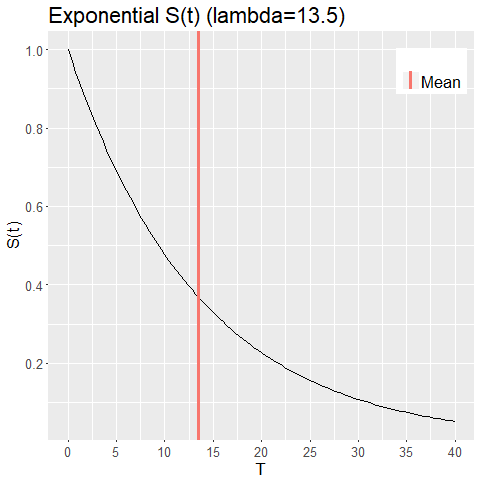
\includegraphics[width=0.98\textwidth]{Figures/expsurv_mean.png}
\column{0.55\textwidth}
\begin{clicker}{The median survival time is \underline{\hspace{0.5in}} the mean survival time of 13.5.}
\begin{enumerate}
\item greater than
\item less than %correct
\item equal to
\item not enough information to determine
\end{enumerate}
\end{clicker}
\end{columns}
\end{frame}

\begin{frame}
\frametitle{Percentiles of $T$}
\begin{itemize}
\item The \textbf{median survival time} is a special case of a \textit{percentile} of the distribution of $T$ (the $50^{th}$ percentile).  This is the time at which 50\% of the individuals have experienced the event.
\item The $p^{th}$ percentile of the distribution of the time-to-event random variable $T$ is the value of $T$, denoted $t_p$ such that:
\item[]
\item[]
\item[]
%\begin{eqnarray}
%\boxed{P(T > t_p)=S(t_p)=1-p/100} \nonumber
%\end{eqnarray}

%    \begin{itemize}
%    \item $P(T<t_p)=p/100$, and;
%    \item $P(T \geq t_p)=1-p/100$, i.e. $\boxed{S(t_p)=1-p/100}$
%    \end{itemize}

\item \textbf{Interpretation}: The $p^{th}$ percentile, $t_p$, can be interpreted as:
\item[] %t_p is the time at which p% of the subjects have already experienced the event, and
\item[] %(100-p)% have not yet experienced the event
\item[] %(100-p)% individuals survive to at least time t_p, and p% of the individuals fail before t_p
\end{itemize}
\end{frame}

\begin{frame}
\frametitle{Graphical representation of percentiles}
\end{frame}

\begin{frame}
\frametitle{Age at first drink: median survival time}
Suppose that the age at first drink of alcohol follows an exponential distribution with parameter $\lambda=13.5$. Find the median age at first drink.  Recall that $S(t)=\exp(-t/\lambda)$.
\vskip150pt
\end{frame}

\begin{frame}
\frametitle{Mean residual lifetime}
\begin{itemize}
\item \textbf{Example: Lung Cancer}. Suppose an individual with lung cancer has survived 100 months since being diagnosed.  Then how much time (on average) does this individual have left to live? We can set this problem up as a \textit{conditional expectation}:
\item[]
\item[]
%E(T-100|T \geq 100)

\item This is an example of quantity known as the \textbf{mean residual lifetime (mrl)}, denoted $\mbox{mrl}(t^*)$, and is
defined to be the average remaining lifetime of all individuals given that the
individuals have survived to time $t^*$, i.e:
\item[]
\item[]
\item[]
\item[]

%\begin{eqnarray}
%\boxed{\mbox{mrl}(t^*)=E(T-t^*|T \geq t^*)=\frac{\int_{t^*}^\infty S(t)dt}{S(t^*)}} \nonumber
%\end{eqnarray}

%\item Suppose a student has completed 6 quarters of college.  How
%many quarters (on average) does this student have left before she
%graduates?
\end{itemize}
\end{frame}

\begin{frame}
\frametitle{Lung cancer example: mean residual lifetime}
If the time until death from cancer follows an exponential distribution with parameter $\lambda=130.18$, then find the average remaining lifetime for those patients who have survived at least 100 days.
\vskip150pt
\end{frame}

%===========================================================================================================================
\section[Evaluating fit]{Evaluating fit}
%===========================================================================================================================
\subsection{}
\begin{frame}
\tableofcontents[currentsection, hideallsubsections]
\end{frame}

\begin{frame}
\frametitle{Considerations for parametric models}
\begin{enumerate}
\item %How do we determine an appropriate probability distribution for $T$
\item[]
\item[]
\item %How do we determine estimates of parameters?
\item[]
\item[]
\item %How do we handle censored event times?
\item[]
\item[]
\end{enumerate}
\end{frame}

\begin{frame}
\frametitle{Veteran's Administration Lung Cancer Study (VALCS)}
\begin{columns}
\column{0.60\textwidth}
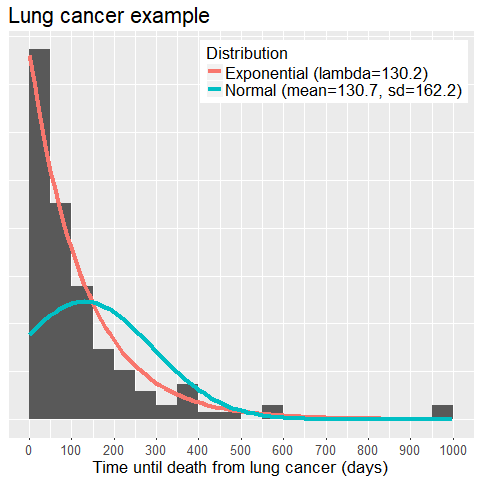
\includegraphics[width=0.98\textwidth]{Figures/veteran_parametric_densities.png}
\column{0.40\textwidth}
Lifetimes (since treatment) of 137 lung cancer patients taken from another lung cancer study with two different probability
density curves superimposed (exponential and normal).
\end{columns}
\end{frame}

\begin{frame}
\frametitle{Strategies for fitting parametric models}
\begin{enumerate}
\item  %fit various density curves, visually identify what is best - can be subjective
\item[]
\item[]
\item %probability plot, e.g., a normal probability plot
\item[] %each observation is plotted against the percentage of observations (roughly) in the sample that is less than or equal to it.  A diagonal line superimposed on the plot represents the cdf of the normal distribution.
\item[] %points along the diagonal line are consistent with the idea that the data come from a normal distribution
\item %conduct a hypothesis test
\item[] %Ho: sample drawn from specified distribution (e.g., normal)
\item[] %Ha: sample not drawn from specified distribution
\end{enumerate}
\end{frame}



\begin{frame}
\frametitle{Probability plots for any distribution}
\begin{itemize}
\item Can construct a probability plot for any distribution
\item With incomplete data, special techniques are used in the probability plot to account for censoring
\item Assess if an exponential distribution fits the data well
\item[]
\begin{itemize}
\item[$H_0$:]
\item[]
\item[$H_a$:]
\item[]
\end{itemize}
\item[]
\begin{enumerate}
\item %visually examine degree of fit of the points to the line
\item[]
\item[]
\item %examine the Anderson-Darling (AD) test statistic
\item[] %small values are weak evidence against H0
\item[] % large values present strong evidence H0
\end{enumerate}
\end{itemize}
\end{frame}

%\begin{frame}
%\frametitle{VALCS study: normal probability plot}
%\begin{columns}
%\column{0.6\textwidth}
%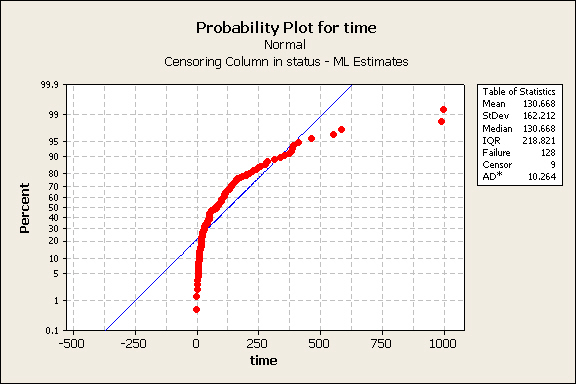
\includegraphics[width=0.98\textwidth]{Figures/norm_probplot_vet.jpg}
%\column{0.4\textwidth}
%\begin{clicker}{Do the data appear to be drawn from a normal distribution?}
%\begin{enumerate}
%\item yes
%\item no %correct
%\end{enumerate}
%\end{clicker}
%\end{columns}
%\end{frame}

\begin{frame}
\frametitle{VALCS study: probability plots}
%\begin{columns}
%\column{0.6\textwidth}
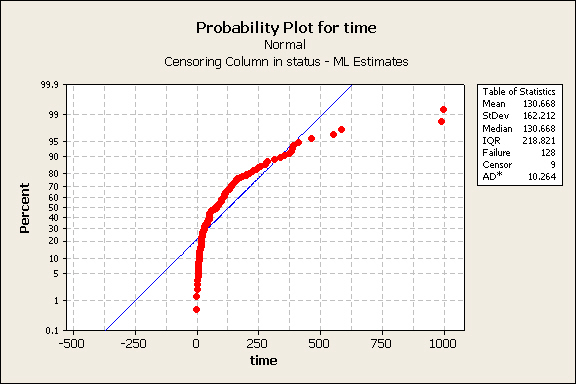
\includegraphics[width=0.49\textwidth]{Figures/norm_probplot_vet.jpg}
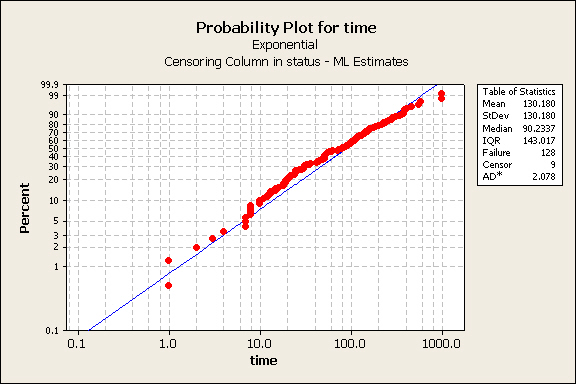
\includegraphics[width=0.49\textwidth]{Figures/exp_probplot_vet.jpg}
\vskip10pt
%\column{0.4\textwidth}
\begin{clicker}{Which distribution appears to fit the data better, and why?}
\begin{enumerate}
\item normal 
\item exponential %correct
\end{enumerate}
\end{clicker}
%\end{columns}
\end{frame}

\begin{frame}
\frametitle{Motorist reaction times: probability plots}
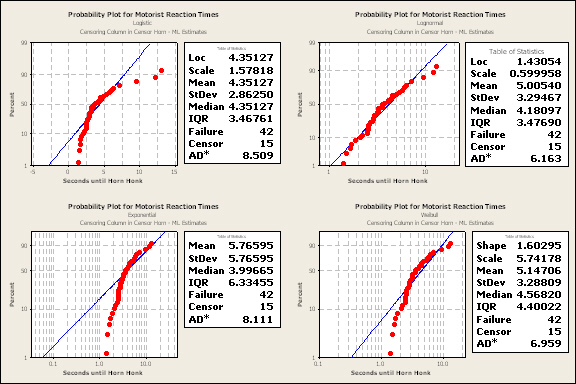
\includegraphics[width=0.95\textwidth]{Figures/prob_plots_motorist.jpg}
%lognormal appears to fit best
\end{frame}


%===========================================================================================================================
\section[Parameter estimation]{Parameter estimation}
%===========================================================================================================================
\subsection{}
\begin{frame}
\tableofcontents[currentsection, hideallsubsections]
\end{frame}

\begin{frame}
\frametitle{Parameter estimation}
\begin{itemize}
\item We have worked through many examples of parametric models for $T$, and in each example, the value(s) of the parameter(s) were given. For example, the time until death for the lung cancer data was assumed to follow an exponential distribution with parameter $\lambda=130.18$.

\item Also, in the previous probability plots (observe the box on the right side), values of the parameters were provided.  How are these values computed?
%based on a sample of event times T1, T2, ... Tn, estimate parameters of a distribution by a using maximum likelihood estimation.
%estimates are called MLEs
\end{itemize}
\vskip100pt
\end{frame}


\begin{frame}
\frametitle{Maximum likelihood estimation}
Suppose we have a random sample of observations $T_1, T_2, \ldots, T_n$ on $n$ individuals, each with the same pdf $f(t_i)$, $i=1, \ldots, n$ and parameter $\theta$ (or possibly more than one parameter).
\begin{itemize}
\item Then \textbf{likelihood function} is given by:
\item[]
\item[]
\item[]
\item[]
\item The likelihood function tells how likely the observed sample is as a function of the parameter values.

\item By \textit{maximizing} the likelihood function, we get the parameter value(s) that most likely would generate our given observed sample.
\end{itemize}
\end{frame}

\begin{frame}
\frametitle{Maximum likelihood estimation, cont.}
\begin{itemize}
\item[Goal:] Find an estimate of $\theta$ that maximizes the likelihood function, $L(\theta)$.
\item[]
\item[Process:]
\begin{enumerate}
\item %find likelihood
\item[]
\item[]
\item %take derivative
\item[]
\item[]
\item %set equation to zero, solve
\item[]
\item[]
\end{enumerate}
\end{itemize}
\end{frame}

\begin{frame}
\frametitle{MLE example: exponential distribution}
Suppose we obtain a random sample of 5 observations, $T_1,T_2,\ldots,T_5$, from an exponential distribution with
parameter $\lambda$ and pdf:
\begin{eqnarray}
f(t) = \frac{1}{\lambda} e^{-t/\lambda} \nonumber
\end{eqnarray}
\begin{enumerate}
\item Construct the likelihood function $L(\lambda)$.
\vskip150pt
\end{enumerate}
\end{frame}

\begin{frame}
\frametitle{MLE example: exponential distribution, cont.}
\begin{enumerate}
\setcounter{enumi}{1}
\item Suppose the observed values of $T_1,T_2,\ldots,T_5$ are $5.3, 4.8, 0.4, 2.3,$ and $0.4$.  Plug these into $L(\lambda)$ and examine the graph of $L(\lambda)$ as a function of $\lambda$.  At which value of $\lambda$ does the likelihood function appear to be maximized?
\item[] 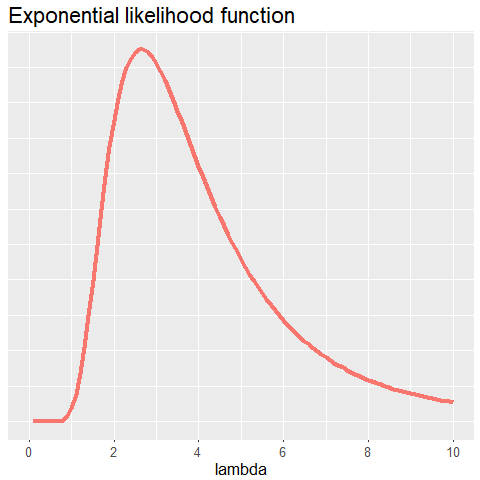
\includegraphics[width=0.50\textwidth]{Figures/exp_likelihood.png}
%appears to maximize around 3
\end{enumerate}
\end{frame}

\begin{frame}
\frametitle{MLE example: exponential distribution, cont.}
\begin{enumerate}
\setcounter{enumi}{2}
\item Find the value of $\lambda$ that maximizes $L(\lambda)$.
\end{enumerate}
\vskip150pt
\end{frame}

\begin{frame}
\end{frame}

\begin{frame}
\frametitle{Likelihood function for right censored data}
If there are right censored event times, then can't simply compute the likelihood function $L$ as the product of
the pdf's. Contributions to the likelihood function differ:
\begin{itemize}
\item If the event time for observation $i$ is complete, then that observation contributes:
\item[] %f(t_i)
\item[]
\item If the event time for observation $i$ is (right) censored, then that observation contributes:
\item[] %S(t_i) = Pr(T>t_i)
\item[]
\item Putting the contributions of all observation together, the likelihood function is given by:
\item[]
\item[]
\end{itemize}
\end{frame}

\begin{frame}
\frametitle{MLE for right censored data}
The following data consist of the times (in months) until relapse of 10 bone marrow transplant patients.  Patients 7-10 were free of relapse at the end of the study.  Suppose time to relapse follows an exponential distribution with parameter $\lambda$.
\begin{center}
\begin{tabular}{c|cccccccccc}
Patient & 1 & 2 & 3 & 4 & 5 & 6 & 7 & 8 & 9 & 10\\ \hline
Relapse Time & 5 & 8 & 12 & 24 & 32 & 17 & $16^+$ & $17^+$ & $19^+$ & $30^+$\\
\end{tabular}
\end{center}
%Construct the likelihood function for the parameter $\lambda$ and find the MLE for $\lambda$.
\begin{enumerate}
\item Construct the likelihood function for the parameter $\lambda$ and find the MLE for $\lambda$.
%\item Assuming that time until relapse follows an exponential probability distribution with $\lambda$ found in Part (1), what is the mean time until relapse?
\end{enumerate}
\end{frame}

\begin{frame}
\frametitle{MLE for right censored data, cont.}
\end{frame}


\begin{frame}
\frametitle{MLE for right censored data, cont.}
\begin{enumerate}
\setcounter{enumi}{1}
\item Assuming that time until relapse follows an exponential probability distribution with $\lambda$ found in Part (1), what is the mean time until relapse?
\end{enumerate}
\vskip200pt
\end{frame}


%===========================================================================================================================
\section[Minitab]{Minitab}
%===========================================================================================================================
\subsection{}
\begin{frame}
\tableofcontents[currentsection, hideallsubsections]
\end{frame}


\begin{frame}[fragile]
\frametitle{Parametric distribution analysis in Minitab}
\begin{itemize}
\item  Along with the probability plots, the MLE's, and summary characteristics about the distribution of $T$ are also computed in Minitab when \texttt{Parametric Distribution Analysis} is performed.

\item The MLE's are provided in the box to the right of the plot, as well as in the output in the Minitab Session Window.

\item The mean, median, quartiles, and several other percentiles are displayed in the Session Window.
\end{itemize}
\end{frame}

\begin{frame}[fragile]
\frametitle{Motorist reaction times in Minitab (lognormal model)}
\begin{verbatim}
    Variable: Seconds until Horn Honk

    Censoring Information  Count
    Uncensored value          42
    Right censored value      15

    Censoring value: Censor Horn = 0
\end{verbatim}
\end{frame}

\begin{frame}[fragile]
\frametitle{Parametric distribution analysis in Minitab, cont.}
\begin{verbatim}
    Estimation Method: Maximum Likelihood

    Distribution:   Lognormal

    Parameter Estimates
                          Standard    95.0% Normal CI
    Parameter  Estimate      Error     Lower     Upper
    Location    1.43054  0.0851775   1.26360   1.59749
    Scale      0.599958  0.0665560  0.482718  0.745673

    Log-Likelihood = -100.729

    Goodness-of-Fit
    Anderson-Darling (adjusted) = 6.163
    ...
\end{verbatim}
\end{frame}

\begin{frame}[fragile]
\frametitle{Parametric distribution analysis in Minitab, cont.}
\begin{verbatim}
    Characteristics of Distribution

                                        Standard   95.0% Normal CI
                              Estimate     Error    Lower    Upper
    Mean(MTTF)                 5.00540  0.500060  4.11529  6.08804
    Standard Deviation         3.29467  0.672961  2.20774  4.91673
    Median                     4.18097  0.356124  3.53813  4.94060
    First Quartile(Q1)         2.78954  0.249485  2.34102  3.32400
    Third Quartile(Q3)         6.26644  0.643405  5.12418  7.66334
    Interquartile Range(IQR)   3.47690  0.541312  2.56254  4.71752
\end{verbatim}
\end{frame}

\begin{frame}[fragile]
\frametitle{Parametric distribution analysis in Minitab, cont.}
\begin{verbatim}
    Table of Percentiles
                         Standard   95.0% Normal CI
    Percent  Percentile     Error     Lower    Upper
          1     1.03545  0.169643  0.751052  1.42753
          2     1.21943  0.181146  0.911401  1.63155
          3     1.35276  0.188314   1.02974  1.77711
    ...
\end{verbatim}
\vskip10pt
\begin{clicker}{What do you think the first line means?}
\begin{enumerate}
\item $Pr(T<1.03545)=0.01$ %correct
\item $Pr(T<1)=0.0103545$
\item $Pr(T>1.03545)=0.01$
\item $Pr(T>1)=0.0103545$
\end{enumerate}
\end{clicker}
\end{frame}

%===========================================================================================================================
\section[Summary]{Summary}
%===========================================================================================================================
\subsection{}
\begin{frame}
\tableofcontents[currentsection, hideallsubsections]
\end{frame}

\begin{frame}
\frametitle{Recap}
\begin{itemize}
\item Features of time-to-event data and survival studies (e.g. censoring, truncation, etc.)
\item Parametric models for the time-to-event random variable $T$: $f(t)$, $F(t)$, $S(t)$, $h(t)$, $H(t)$
\item Descriptive measures for $T$: $E(T)$, $t_p$, and, $\mbox{mrl}(t^*)$
\item Strategies for selecting a probability model: probability plots, AD test statistic
\item Parameter estimation: maximum likelihood estimation
\end{itemize}
\end{frame}


\begin{frame}
\frametitle{Future}
\textbf{Nonparametric} methods for summarizing and describing samples of time-to-event data:
\begin{itemize}
\item[]
\item Estimators for $S(t)$, $h(t)$, and $H(t)$.
\item Estimates of $E(T)$ and $t_p$
\item Inference methods for the estimator of $S(t)$
\item Inference procedures for comparing two or more survival experiences.
\item Survival analysis in R
\end{itemize}
\end{frame}

\end{document} 